\section{Revisiting Square Data}

\begin{frame}{Revisiting Square Data}
    \begin{itemize}
        \item Revisit the square data set to see if there are similar patterns
        \item Construct a data set similar to the ellipse set with pre- and post-impact data
        \item Use visualizer to manually determine if the data is "good"
        \item Detect a collision if $\dot{y}$ goes from negative to positive and $y_{com}$ is at a local minimum
    \end{itemize}
\end{frame}

\begin{frame}{Example of Visualizer}
    \centering
    \animategraphics[controls, width=\linewidth / 3*2] {12}{gifDrop/frame-}{0}{74}
    \\
    \centering
    Trial 20
\end{frame}

\begin{frame}{Extracting Velocities}
    \begin{itemize}
        \item Noise in the position measurements can lead to extremely inaccurate velocity calculations
        \item  Amplified by the time step ($v_1 = \frac{x_0 + x_1}{dt}$)
        \item Most common solution is a filter
    \end{itemize}
    
\end{frame}

\begin{frame}{Extracting Velocities}
    \begin{itemize}
        \item Fit lines to pre- and post-impact data to improve accuracy
        \item Helps adjust for bad data points and inaccuracies due to any filters applied
        \item Extract velocities from slopes of position curves
    \end{itemize}
    
    \begin{figure}[h!]
        \centering
         \begin{subfigure}[b]{0.45\linewidth}
                \centering
                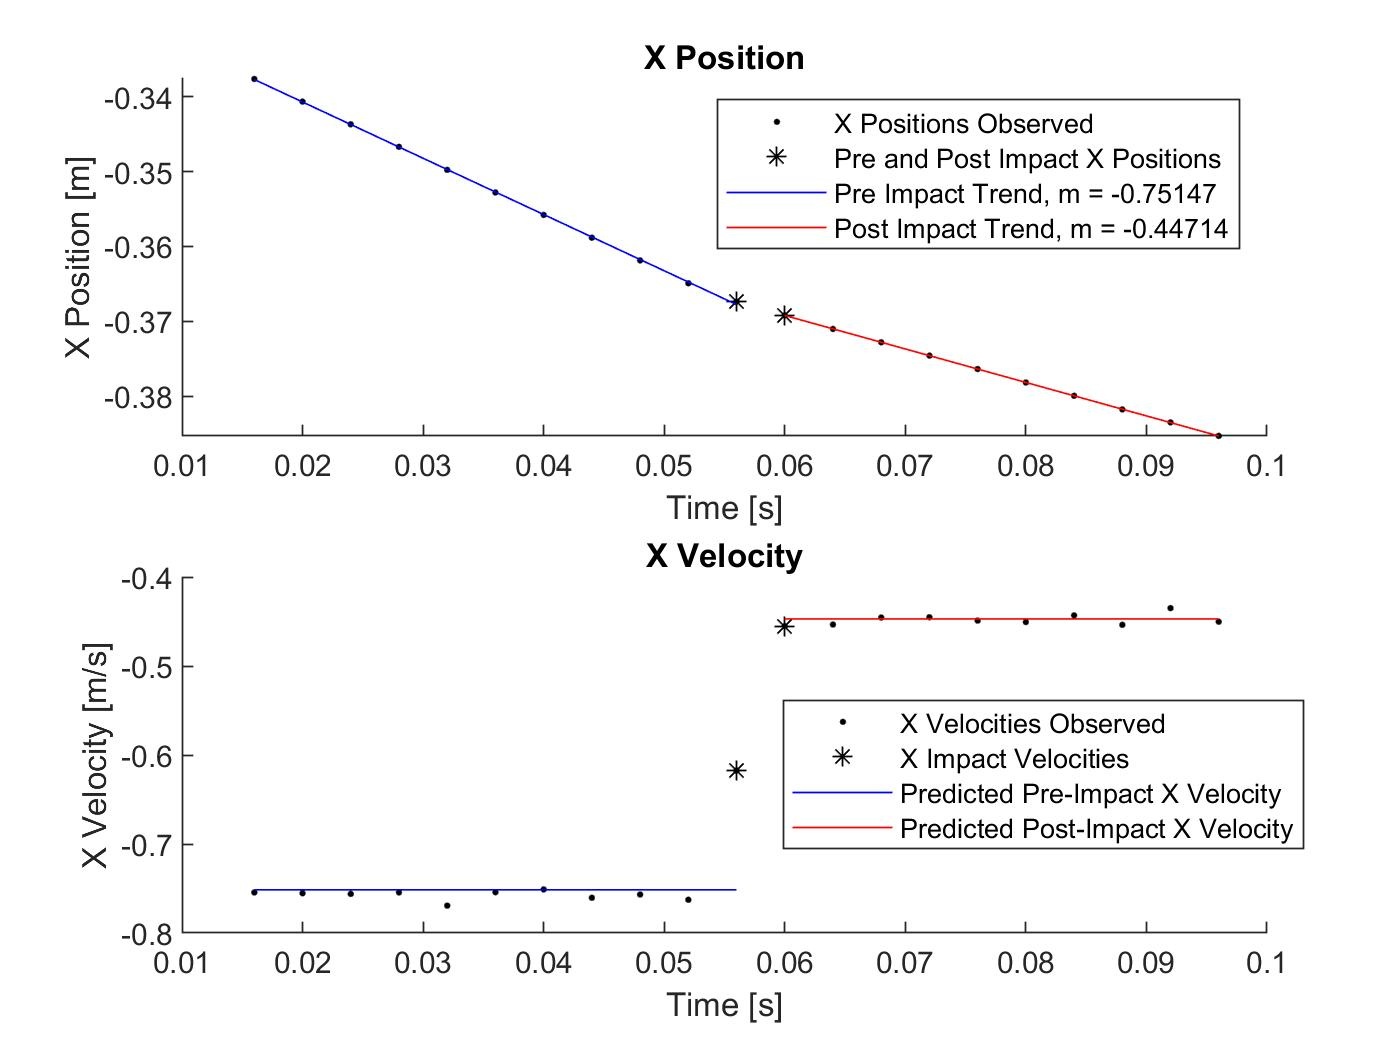
\includegraphics[scale=0.09]{figures/xTrial6.jpg}
                \caption{X Position and Velocity}
                \label{fig:xt6}
        \end{subfigure}
        \begin{subfigure}[b]{0.45\linewidth}
                \centering
                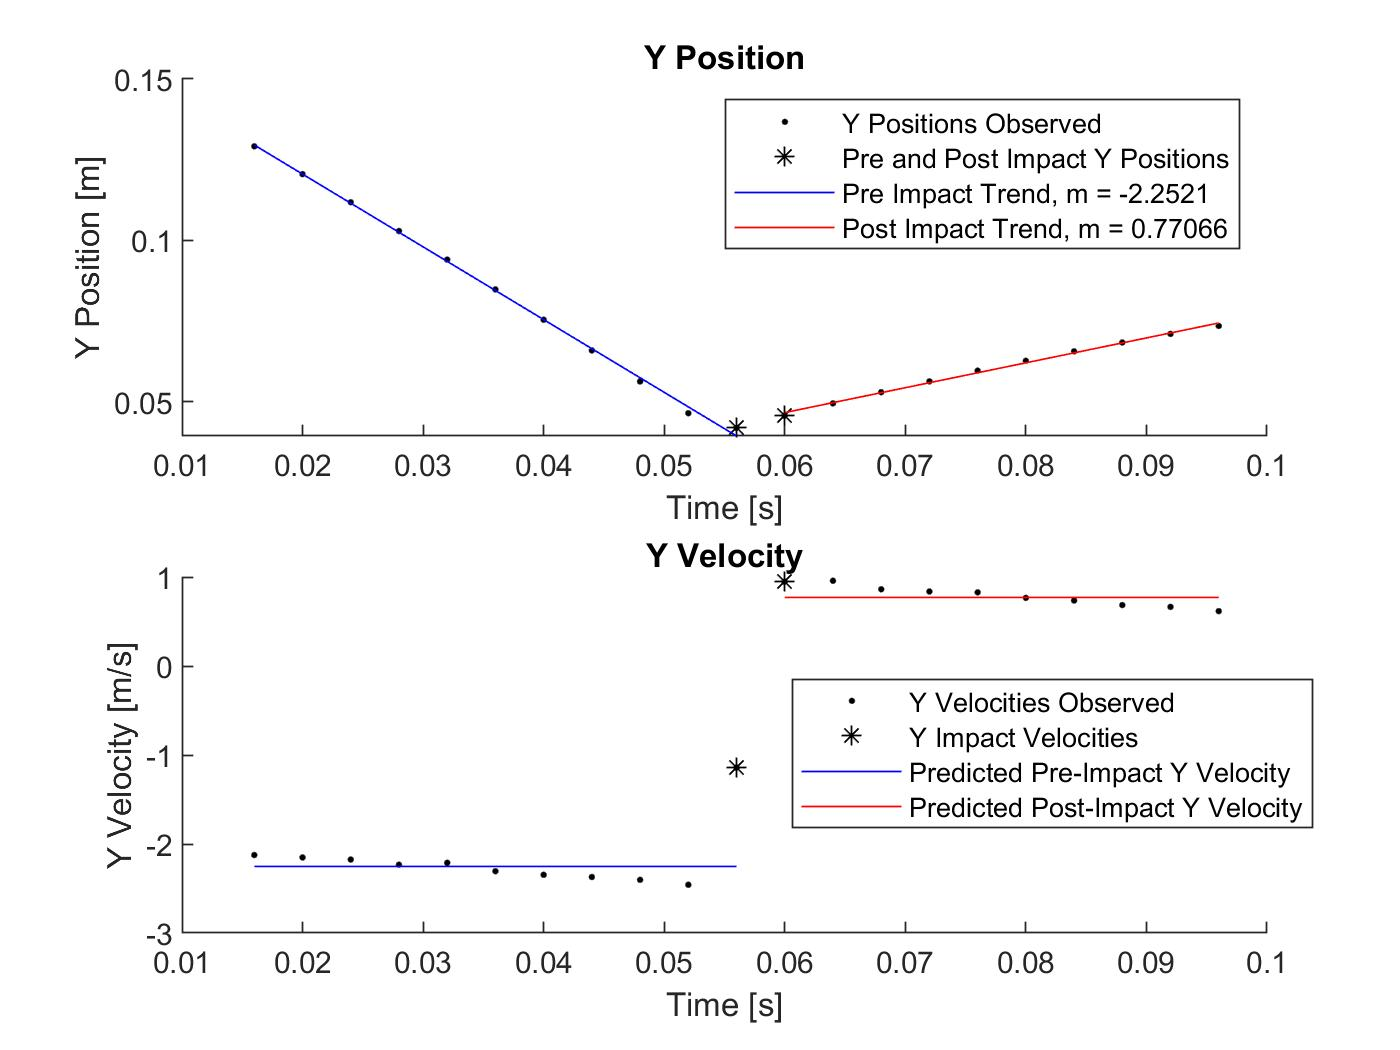
\includegraphics[scale=0.09]{figures/yTrial6.jpg}
                \caption{Y Position and Velocity}
                \label{fig:yt6}
        \end{subfigure}
        \vspace{-1\baselineskip}
        \caption{Finding Pre- and Post-Impact Velocity for Trial 6}
    \end{figure}
\end{frame}

\begin{frame}{Effect of Fitting Velocity}
    \begin{figure}[h!]
        \centering
         \begin{subfigure}[b]{0.45\linewidth}
                \centering
                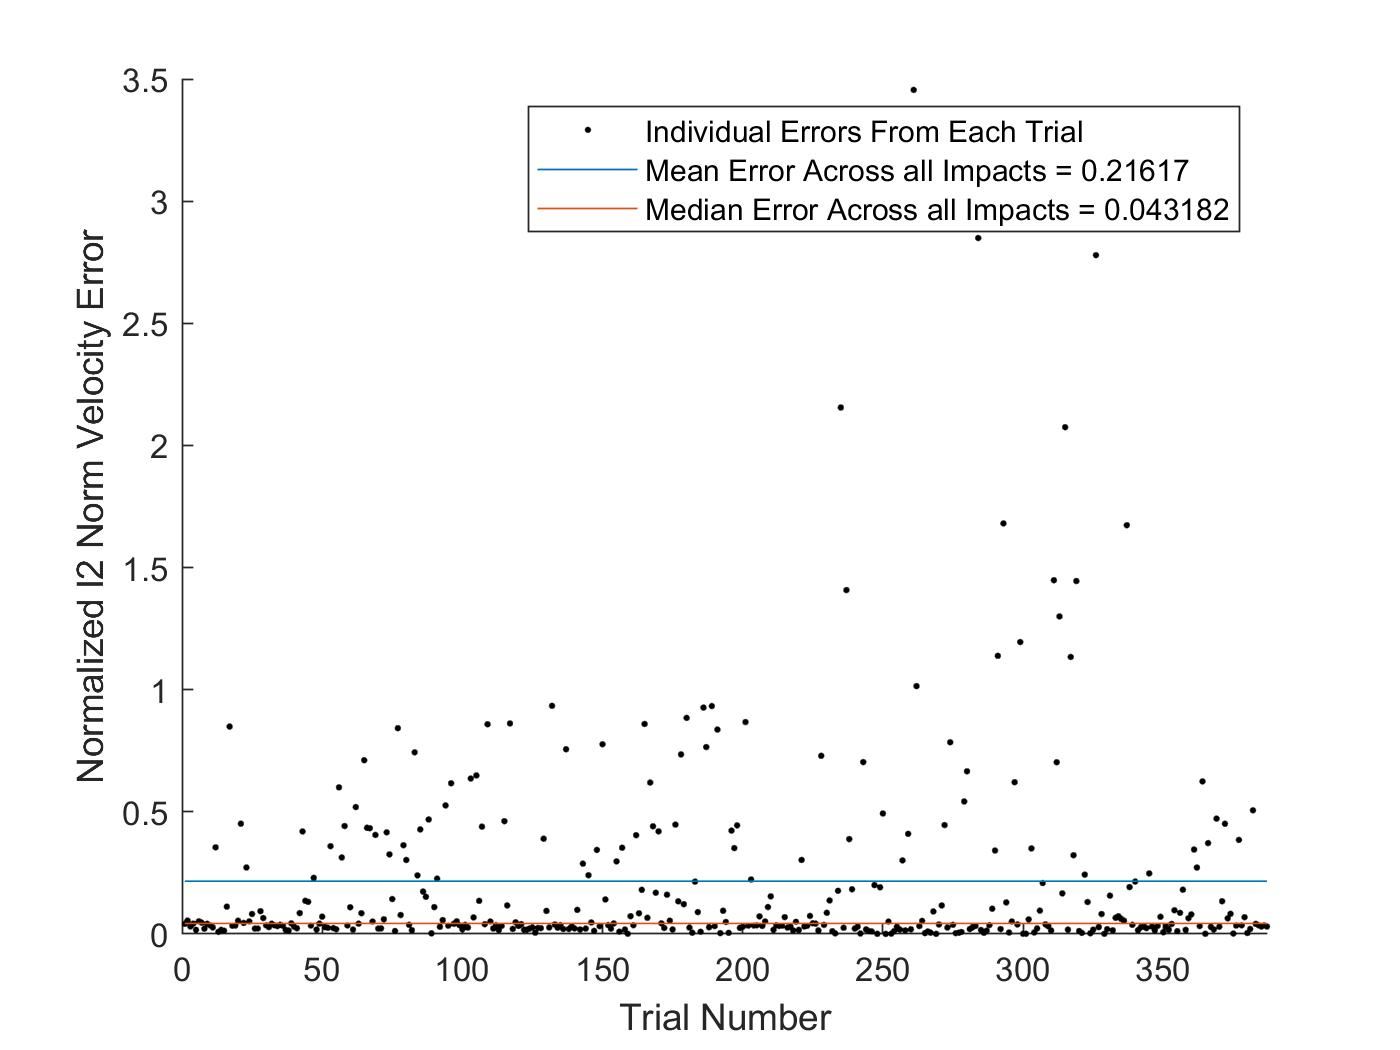
\includegraphics[scale=0.1]{figures/OriginalSquareData.jpg}
                \caption{Taking Velocities Directly}
                \label{fig:OrigSD}
        \end{subfigure}
        \quad
        \begin{subfigure}[b]{0.45\linewidth}
                \centering
                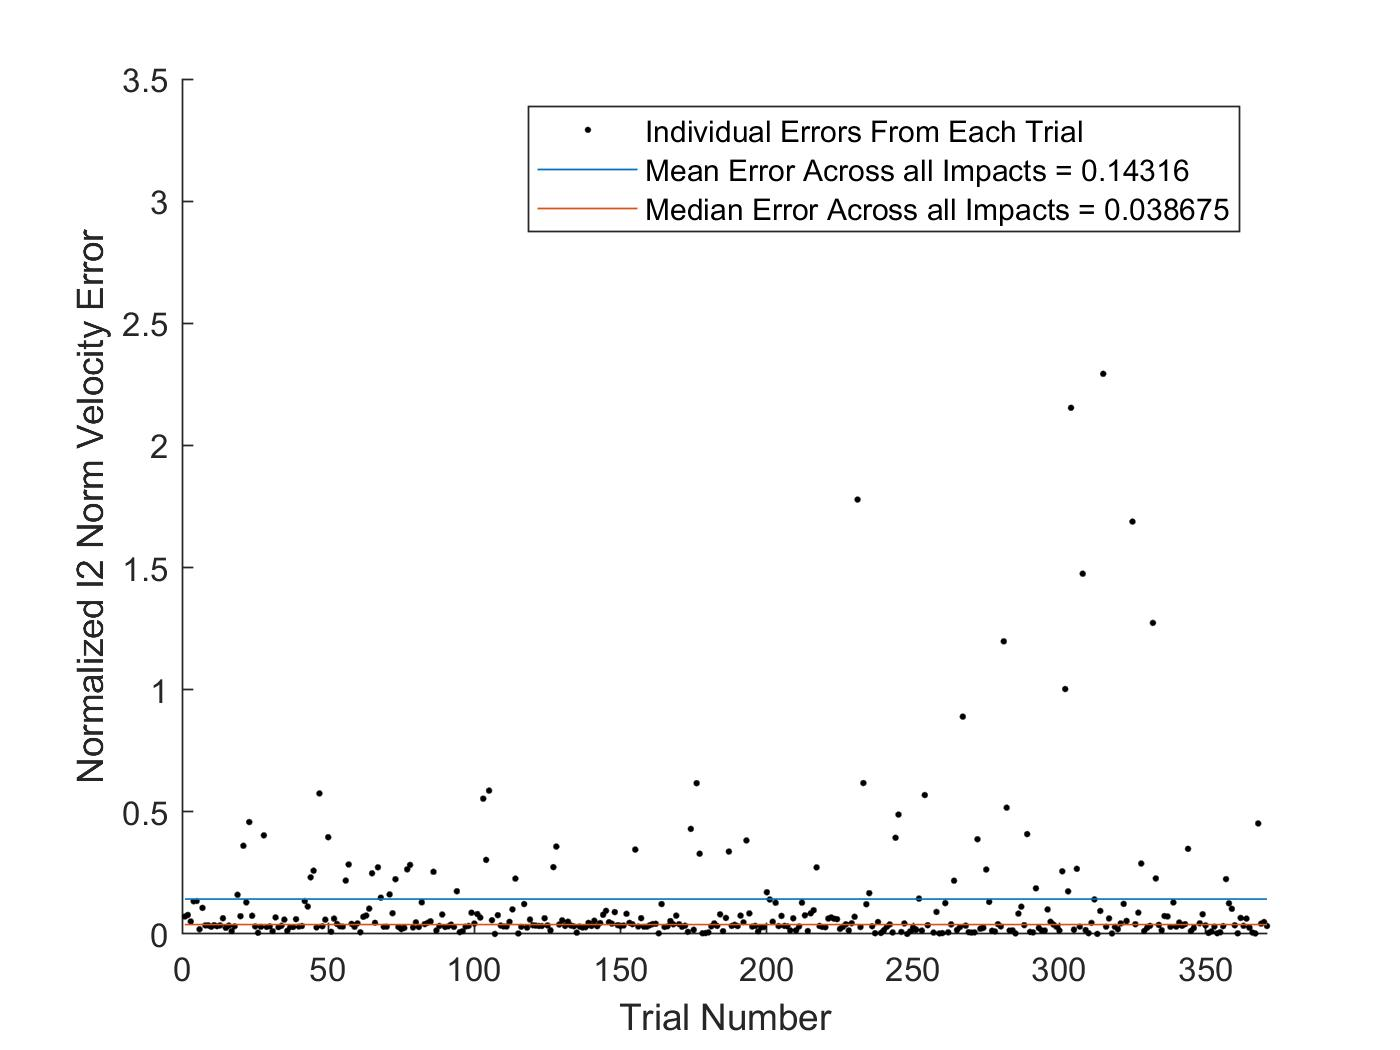
\includegraphics[scale=0.1]{figures/updatedSquareData.jpg}
                \caption{Using Fitted Velocities}
                \label{fig:UpdatedSD}
        \end{subfigure}
        \caption{Comparing Accuracy of IRB Model for Adjusted Data Set with Velocities Extracted from Fitted Position Curves}
    \end{figure}

\end{frame}

\begin{frame}{Results: Comparing provided data vs simulated data}
 \vspace{0.5\baselineskip}
One last thing that we tried was to see whether the simulated data set (using pybullet) that Dr. Fazeli had available on git would make a difference in the error of the IRB model. Below we present our results:

\begin{figure}
    \centering
    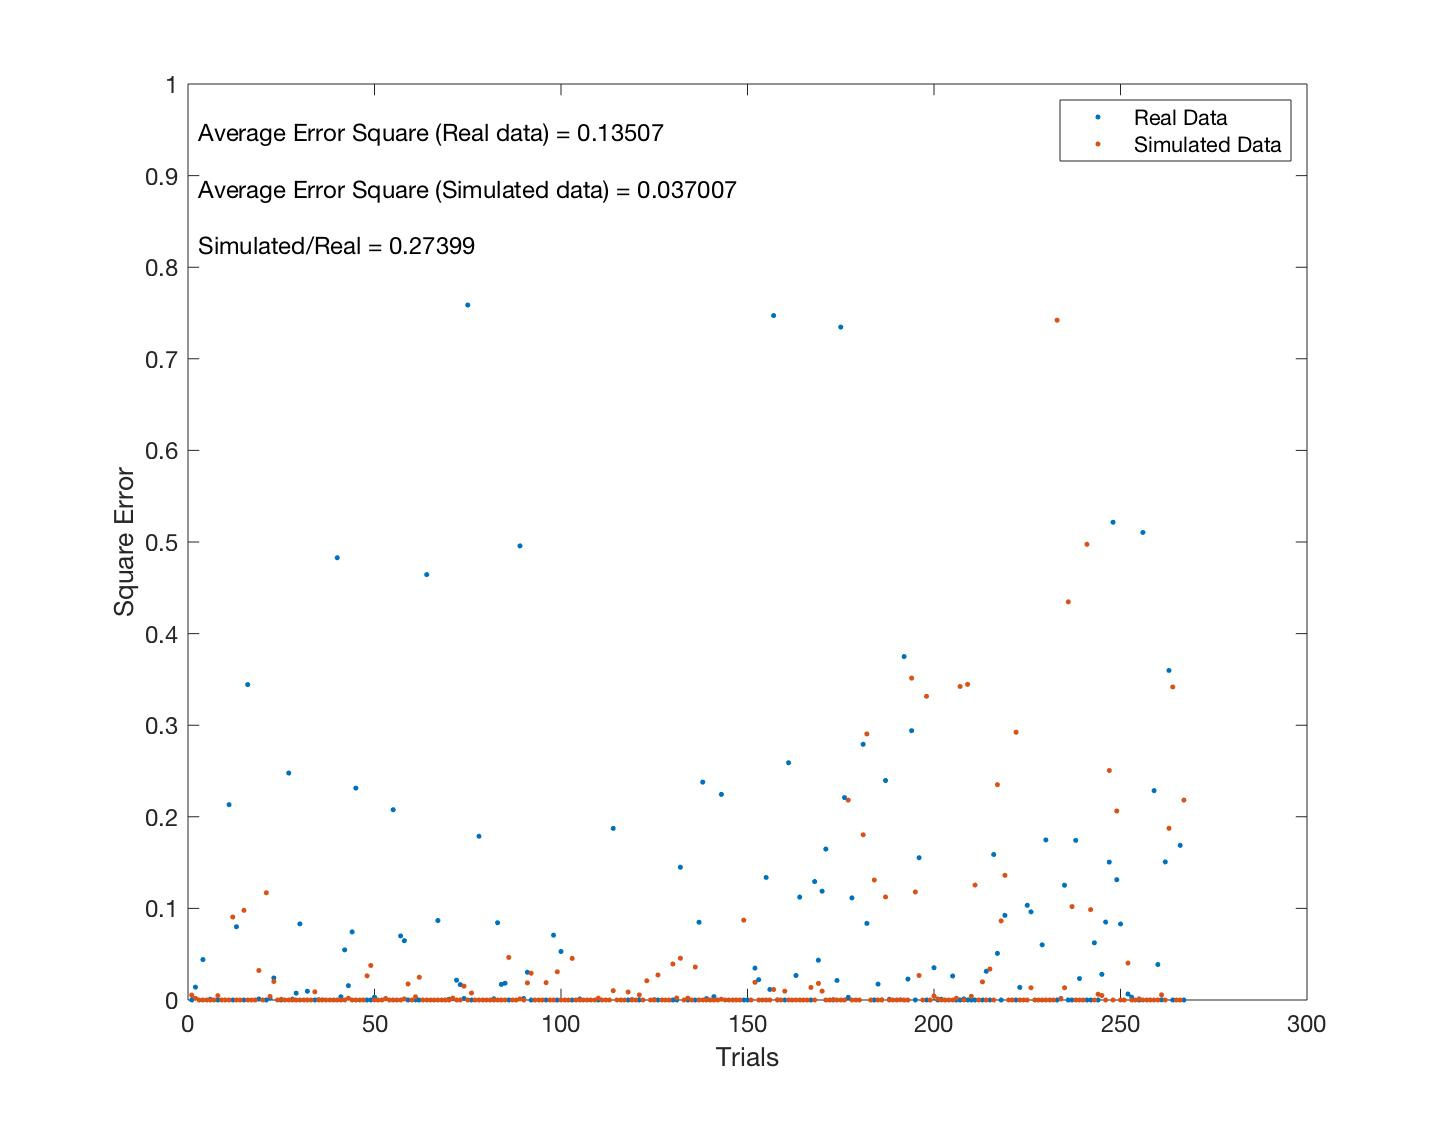
\includegraphics[scale=0.14]{figures/SquareDataErrorSimulated.jpg}
    \caption{Provided vs Simulated Data error}
    \label{fig:MomentsError}
\end{figure}

\end{frame}